\documentclass[11pt]{article}
\usepackage[utf8]{inputenc}

\usepackage{graphicx,amsmath,amsfonts,amssymb,fullpage, color,natbib,url}
% Keywords command
\providecommand{\keywords}[1]
{\small	
  \textbf{Keywords}: #1}
\newcommand{\argmax}{\operatornamewithlimits{argmax}}
\newcommand{\argmin}{\operatornamewithlimits{argmin}}

\title{\textbf{Policy compression: an information bottleneck in action selection}}
\author{Lucy Lai$^{1,\ast}$, and Samuel J. Gershman$^{2}$ \\
$^1$Program in Neuroscience, Harvard University \\
$^2$Department of Psychology and Center for Brain Science, Harvard University \\
$^\ast$Correspondence: lucylai@g.harvard.edu}
\date{}

\begin{document}

\maketitle
\tableofcontents

\begin{abstract}
   The brain has evolved to produce a diversity of behaviors under stringent computational resource constraints. Given this limited capacity, how do biological agents balance reward maximization against the costs of representing complex action policies? In this chapter, we examine behavioral evidence for this reward-complexity trade-off. First, we introduce a theoretical framework that formalizes the idea of \emph{policy compression}, or the reduction in cognitive cost of representing action policies by making them simpler. We then describe how a wide range of behavioral phenomena, including stochasticity, perseveration, response time, state and action chunking, and navigation are brought together under this framework. Finally, we discuss how our model can be used to probe the neural underpinnings of policy compression and their dysfunction in psychiatric illness.
\end{abstract}

\keywords{action selection, reinforcement learning, rational behavior,  resource-rationality}

\section{Introduction}

All action demands memory. When you go shopping, drive to work, or prepare a meal, your brain is retrieving stored information about \emph{policies}, the mappings from states of the world to actions. Like all mappings in the brain, policies are capacity-limited: a finite physical storage medium imposes an upper bound on the number of bits (the description length) that can be used to specify policies. The need to economize on description length means that policies should be compressed as much as possible, discarding redundant bits and reducing precision where it's not needed. We will shortly formalize policy compression, but first we provide some intuitions.

Imagine you are preparing a meal for your family. In this case, states correspond to family members, actions correspond to dishes, and policies are mappings from family members to dishes (Figure \ref{fig:diagram}). If you're lucky, everyone in your family will eat the same thing. This means that you can ignore the state entirely and just take the same action (prepare the same dish) repeatedly. Such a policy is compressed in the sense that it consumes fewer bits of memory compared to one in which you need to remember separate dishes for each family member. This illustrates the concept of \emph{redundancy reduction}: remembering separate dishes would be redundant because they would simply be copies of the same dish. Remembering a single dish for everyone eliminates this redundancy.

If you are a mentally taxed parent, you might need to compress your policies more aggressively. Your children won't be able to tell the difference between Greek and Italian olive oil, so there's no need to distinguish between dishes that differ in that one ingredient. Just choose randomly! A random policy requires fewer bits than a deterministic policy, because you no longer need to remember which action to take in a particular state. Similarly, it's not worth spending bits on a policy for the teenager who rarely shows up at dinner; you can safely compress your policy by choosing randomly. These examples illustrate the concept of \emph{precision reduction}: compression can be achieved by forgetting distinctions that don't matter.

The idea of compression has played an important role in theories of short-term memory \citep{miller56,brady09,nassar18,mathy12,norris20}, but until recently it has been comparatively neglected in theories of action selection. Despite this neglect, we will show that many aspects of action selection (stochasticity, perseveration, response time, and chunking) can be viewed as forms of policy compression. To set the stage, we will begin by introducing a general information-theoretic framework for understanding compression, adapted from applications to memory and perception research \citep{gershman21,sims16}. This will allow us to derive the optimal policy under a given capacity constraint and deduce empirical predictions from this policy.

\section{Action selection as a communication channel}

At first glance, it is somewhat counter-intuitive to think of action selection in terms of communication; in what sense are actions communicating anything? To understand why this makes sense, let us first consider memory more broadly as a channel for transmitting information about the past for use in the future. In the same way, selecting an action requires transmitting information about states to guide future action. 

In our running example, this means that while you are cooking, you must be able to remember \textit{who} will be at dinner (state) in order to know what dish (action) to cook for each family member. Similarly, cooking a particular dish (action) provides information about the particular family member (state) you are serving. Note that the current state might include features of the past (e.g., stimuli, actions, rewards, etc.), and hence it is appropriate to think of the state as a kind of historical record or summary statistic.\footnote{In reinforcement learning theory \citep{sutton18}, ``state'' has a technical meaning related to Markov decision processes: the state is a sufficient statistic for predicting future states and rewards. In other words, an agent can forget the past once it knows what state it's currently in.} (For example, a ``feature'' of your teenager is that they rarely show up at dinner.) 

Unfortunately, our brains are \textit{not} perfect at remembering all of the state information needed to guide action. A distracted or tired chef might misremember who wants to eat what dish, and may even confuse preferred dishes between family members. In other words, there are capacity limits on memory that constrain the amount of information that can be faithfully transmitted. Viewing action selection as a communication channel allows us to formalize these capacity limits using the language of information theory. From this foundation we can analyze the structure of optimal policies under capacity limits, and derive practical algorithms for policy compression.

As diagrammed in Figure \ref{fig:diagram}A, the channel input is generated by a distribution $P(s)$ over states ($s$). The channel encodes each state into a \emph{codeword} $c$; this is the step at which compression occurs, as we discuss below. Conditional on the codeword, the channel selects an action $a$ according to $P(a|c)$. Taken together, these two steps (encoding and action selection) produce the policy $\pi(a|s)$ mapping states to actions. An illustration of these steps using our running example is shown in Figure \ref{fig:diagram}B.

\begin{figure}
    \centering
    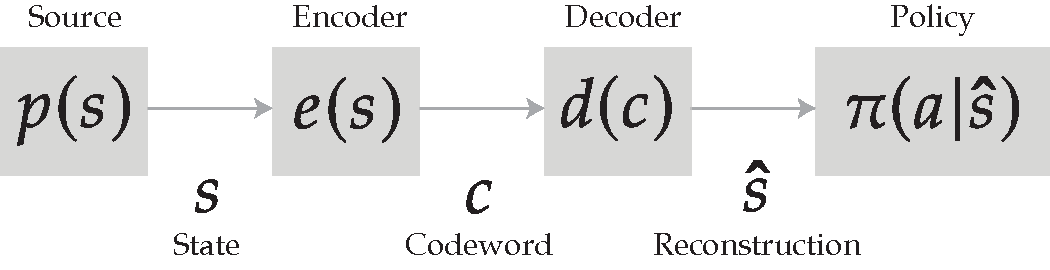
\includegraphics[width=\textwidth]{figs/diagram.pdf}
    \caption{\textbf{The policy as a communication channel.} (A) We start with an distribution $P(s)$ over states ($s$). Each state is encoded into memory via an \textit{encoder}, $e(s)$, yielding a codeword $c$. The codeword is then mapped onto an action $a$ according to $P(a|c)$. Together, encoding and action selection produce the policy $\pi(a|s)$ mapping states to actions. (B) Imagine three family members (states) at dinner that a chef must account for. Each family member can be represented by a codeword, whose length is constrained by the chef's capacity limit (measured in bits). This corresponds to the amount of memory they have allocated to remembering relevant information about family members (e.g., whether they have a preferred dish, have dietary restrictions, etc.). The codeword representations are used to select the dishes (actions) that the chef will cook. (Top) In the case where the chef has 2 bits of memory at allocate, they can differentiate between family members' food preferences. (Bottom) However, when the chef can only allocate 1 bit of memory to the family member-dish mapping, they do not differentiate between food preferences and end up making the same dish for everyone.}
    \label{fig:diagram}
\end{figure}

Compression can be quantified in terms of the state's description length, the length of the codeword. Since we can always translate the codeword into binary strings of 0's and 1's (bits), we can compare the description lengths of codewords in units of bits. The channel capacity places a limit on the average description length of codewords. In particular, the minimum number of bits needed for error-free transmission of the state identity is given by the mutual information between states and actions \citep{shannon48}:
\begin{align}
    I(S;A) = \sum_{s} P(s) \sum_{a} \pi(a|s) \log \frac{\pi(a|s)}{P(a)},
\end{align}

In the context of action selection, we will refer to the information rate as the \emph{policy complexity} because policies that are more highly state-dependent (i.e., action probabilities vary to a greater degree across states) require on average more bits to encode. For instance, a policy in which you have to make different dishes for each family member is more complex than one in which you can make the same dish for everyone.

There are a number of complementary ways to understand policy complexity. Suppose you observe only the inputs (states) to the channel; how much do these observations help you predict the outputs (actions)? Policy complexity is mathematically equivalent to the reduction in uncertainty about the actions conditional on the states:
\begin{align}
    I(S;A) = H(A) - H(A|S),
\end{align}
where
\begin{align}
    H(A) = -\sum_a P(a) \log P(a)
\end{align}
is the entropy of the marginal action distribution, expressing uncertainty about the actions prior to observing the states, and
\begin{align}
    H(A|S) = -\sum_s P(s) \sum_a \pi(a|s) \log \pi(a|s)
\end{align}
is the conditional entropy, expressing the uncertainty about the actions after observing the states, averaged over the action distribution. Intuitively, knowing \textit{who} a distracted (low capacity) chef is currently cooking for provides relatively little information about \textit{what} they are going to serve.

We can also understand policy complexity as the degree of uncertainty reduction about the inputs conditional on the outputs:
\begin{align}
    I(S;A) = H(S) - H(S|A).
    \label{eq:infrate}
\end{align}
In other words, if I only observe an agent's actions, policy complexity measures how well I can infer the unobserved state driving those actions. Watching a distracted chef prepare dishes provides relatively little information about \textit{whom} they are about to serve.

\section{Compression as a trade-off between reward and complexity}

In this section, we consider the channel design problem: how should the brain optimize for accurate encoding and decoding with the goal of minimizing distortion (or equivalently, maximizing reward), given capacity limitations? First we need to clarify what it means to be optimal. If the goal is lossless (error-free) transmission, then the goal is to choose an encoder that achieves the Shannon bound, with average description length equal to the information rate. If there is no channel noise, the inputs can be unambiguously inferred from the outputs, and hence the conditional entropy $H(S|A)$ is 0. According to Eq. \ref{eq:infrate}, the policy complexity is then equal to the source entropy, $H(S)$. The shortest average description length is thus also equal to the source entropy.\footnote{This is an informal statement of Shannon's source coding theorem \citep{shannon48}.}

The optimal error-free code under noiseless transmission can be achieved by a family of algorithms known as \emph{entropy coding}, which assign codewords to each state $s$; the codeword's length (in bits) is equal to the state's \emph{surprisal}, $-\log P(s)$. In fact, the expected surprisal is equal to the source entropy, thus satisfying the Shannon bound. The canonical algorithm for entropy coding is Huffman coding \citep{huffman52}, which constructs a binary tree whose leaf nodes correspond to input symbols (states). The binary code for each state can be thought of as a sequence of instructions for traversing the tree and terminating at a leaf node to reveal the encoded state. This decoding procedure has interesting implications for understanding response time, as we will see later.\footnote{See \citet{brady09} and \citet{norris20} for further examples of studies that use Huffman coding as a psychological model.}

The basic problem with error-free transmission as a theory of action selection is that the brain is not, and cannot, be error-free. As was recognized long ago by \citet{vonneumann58}, the brain is a low precision communication system, corrupted by many sources of noise \citep[see][for a contemporary review]{faisal08}. Thus, a compression scheme like Huffman coding, which eliminates all redundancy, is \emph{prima facie} implausible. In unreliable communication systems like the brain, redundant bits are needed to correct transmission errors \citep{bhui18,tkavcik10}. However, if capacity is too low, there will not be sufficient bits available to correct all errors. This raises the question: how should the brain allocate bits when there are not enough to go around?

Rate-distortion theory was developed to answer this question \citep{berger71}.  The key idea is that bits should preferentially go to transmitting information that matters. Applied to action selection, the theory stipulates a distortion function $d(s,a)$ that measures the cost of outputting $a$ when the state is $s$.\footnote{Traditionally, the channel output is conceived as a reconstruction of the state, so that distortion refers intuitively to the difference between the input and reconstruction. Thus, the term ``distortion'' is somewhat confusing in the context of action selection, where we take it to mean the cost function.} The optimization problem is to minimize the expected distortion $D = \mathbb{E}[d(s,a)]$ subject to a constraint on the information rate, or equivalently minimize the information rate subject to a constraint on the expected distortion. In the context of action selection, it is often more natural to work with the reward $Q(s,a)$, the mirror image of the distortion. The application of rate-distortion theory to action selection has been developed theoretically by a number of different authors \citep{tishby11,parush11,lerch18,fox15,still12,grau18}. Our summary of these ideas is condensed and simplified (for example, we do not address sequential decision problems), so the interested reader is referred to these papers for more technical details.

It can be shown that the highest achievable expected reward for a given capacity constraint is a monotonically increasing and concave function of policy complexity (see Figure \ref{fig:gershman20}). There is thus a trade-off between reward and policy complexity: greater compression of states (lower complexity) can only be achieved at the expense of reward. In subsequent sections, we will explore the empirical implications of this trade-off.

A number of these implications can be deduced from the functional form of the optimal policy:
\begin{align}
    \pi^\ast(a|s) = \frac{\exp[\beta Q(s,a) + \log P^\ast(a)]}{\sum_{a'} \exp[\beta Q(s,a') + \log P^\ast(a')]}.
    \label{eq:optimalpolicy}
\end{align}
This is the familiar softmax equation, ubiquitous in studies of reinforcement learning, psychophysics, and econometrics. The parameter $\beta$ is commonly referred to as the \emph{inverse temperature}, and controls the degree of stochasticity; as $\beta$ increases, the policy concentrates on the action with highest reward. In rate-distortion theory, $\beta$ has another interpretation; its inverse (the temperature) is the slope of the reward-complexity trade-off function:
\begin{align}
    \beta^{-1} = \frac{d V}{d I(S;A)},
    \label{eq:beta}
\end{align}
where $V = \mathbb{E}[Q(s,a)]$ is the expected reward. The second term inside the softmax,
\begin{align}
    \log P^\ast(a) = \log \sum_s P(s) \pi^\ast(a|s),
\end{align}
captures a form of perseveration, a bias towards actions that are chosen frequently across all states. Low complexity policies compress the state and therefore cannot distinguish between policies for different states. As a consequence, the optimal policy will be close to the marginal distribution over actions, ignoring the state (see empirical examples from Figure \ref{fig:gershman20}).

How can we actually compute the optimal policy? Notice that the perseveration term depends on the optimal policy, so there is a circularity in the definition. The Blahut-Arimoto algorithm \citep{blahut72,arimoto72} harnesses this circularity by iterating between computing $P(a)$ and $\pi(a|s)$, a process that will converge to the optimal values.

One drawback of the Blahut-Arimoto algorithm is that computing $P(a)$ requires a marginalization over the entire state space. If the state space is very large or continuous (as in many real-world environments), this marginalization might be computationally intractable. In the Appendix, we derive a tractable algorithm based on a reinforcement learning formulation \citep[see also][]{gershmanlai20}. This algorithm incrementally modifies the policy based on reward feedback, with the critical property that the agent is penalized for complex policies. While the algorithm will eventually converge to the optimal policy, its incremental nature means that it will spend a non-trivial amount of time away from the optimal trade-off curve. We will later show that this allows it to explain empirical deviations from the optimal curve.

\section{Behavioral signatures of policy compression}

In the following sections, we review behavioral phenomena that can be interpreted in terms of policy compression. For some of these phenomena, we present illustrative simulations using the process model presented in the Appendix. Our goal is synthetic rather than discriminative: although each individual phenomenon may be explained by alternative theories, we make the case that they can be understood collectively as reflections of a single underlying principle.

\subsection{Stochasticity}
Imagine that you are shopping for wine at the grocery store. You don’t know much about wine, so you select one at random and later discover that you like it. However, when you return to the wine aisle the next week, you decide to randomly select a different wine instead of picking the one you chose last time. This example illustrates the stochasticity inherent in our daily choice behaviors.
 
Why are human actions stochastic even when faced with the same choice options? There are a number of different answers to this question \citep[see][]{icard19}. One conventional answer in the framework of reinforcement learning is that stochasticity facilitates exploration \citep{schulz19}. In order to identify the most rewarding action, an agent must sample multiple actions, and injecting randomness into the policy (e.g., via the softmax equation) is a simple way to accomplish this. However, the exploration perspective does not explain why action selection is apparently stochastic even in situations where the payoffs and probabilities are fully known \citep[e.g.,][]{mosteller51}. In economics, a standard explanation of stochasticity is the hypothesis that actions are evaluated based on a random utility function that specifies a level of inherent randomness when sampling actions in proportion to their expected payoffs. But this just pushes the question back further: why is the utility function random?

The results from rate-distortion theory presented earlier provide a different foundation for stochastic action selection. Any capacity-limited agent must be stochastic if they are operating at the optimal reward-complexity frontier. Remarkably, this optimal stochasticity should take the form of a softmax policy, consistent with the way in which psychologists and economists have long modeled action selection.\footnote{The softmax policy is known as the multinomial logit policy in economics; see \citet{mcfadden01}.} In the economics literature, this insight was derived within the framework of ``rational inattention'' \citep{matvejka15}, which is mathematically equivalent to the Lagrangian formulation of the rate-distortion objective function \citep[see Appendix and][]{denti19}.

Rate-distortion theory not only rationalizes the softmax policy; it also links the temperature (commonly treated as a free parameter that is fit to data) as a function of the reward-complexity trade-off. Specifically, Eq. \ref{eq:beta} shows that the temperature corresponds to the slope of the reward-complexity trade-off function. Because the trade-off function is concave, and hence the slope is monotonically decreasing in the policy complexity, the optimal policy is more stochastic for low complexity policies.

\begin{figure}
    \centering
    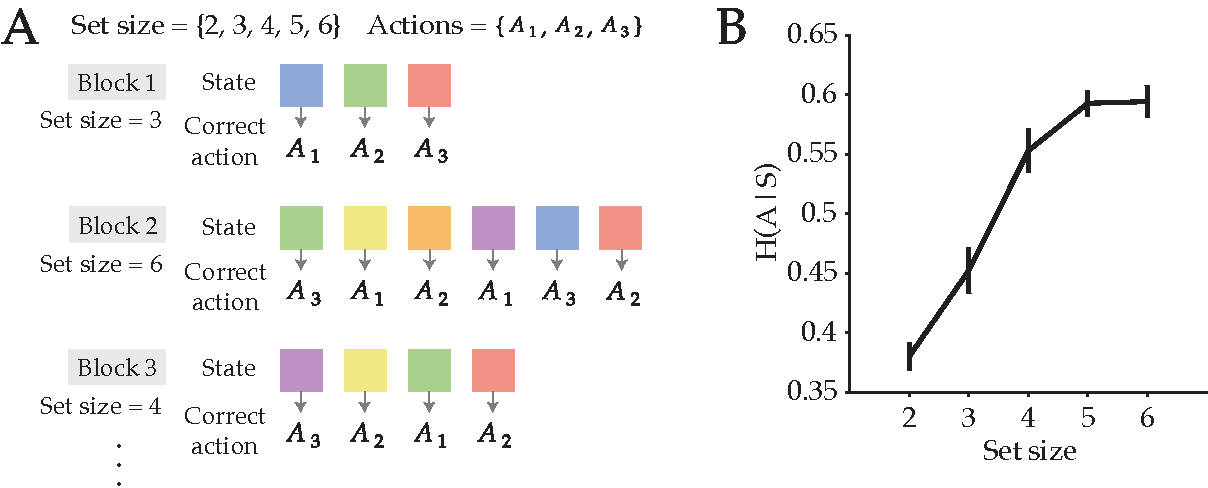
\includegraphics[width=0.9\textwidth]{figs/entropy.pdf}
    \caption{\textbf{Stochasticity as a function of set size.} (A) In the task developed by \cite{collins12}, subjects saw a single stimulus on each trial and chose between 3 actions. Each stimulus had a single rewarded action. The number of states, or set size, varied between 2 and 6 across blocks.  (B) Conditional entropy as a function of set size in data from healthy controls in \citet{collins14}. Error bars show standard error of the mean.}
    \label{fig:stochasticity}
\end{figure}

One implication is that increasing cognitive load, which should reduce policy complexity or force a fixed complexity to be distributed across more states, will cause action selection to be more stochastic. \citet{collins12} developed an experimental paradigm, a kind of ``contextual multi-armed bandit'' task, that allows us to test this hypothesis (Figure \ref{fig:stochasticity}A). In their experiment, subjects were shown a stimulus (the state variable in our terminology) and were tasked with selecting one of 3 actions. If they chose the correct action, they were rewarded. Critically, the number of states (the set size) was manipulated across blocks. Collins and Frank reported that performance degraded with set size. If an agent's policy complexity decreases with set size, or if the policy complexity is distributed across more states, then we should expect higher stochasticity for larger set sizes. Using the conditional entropy $H(A|S)$ as a measure of stochasticity, this prediction is confirmed (Figure \ref{fig:stochasticity}B).\footnote{This analysis used data from a follow-up study \citep{collins14}, which we have previously re-analyzed \citep{gershmanlai20}.}


\subsection{Perseveration}

\begin{figure}
    \centering
    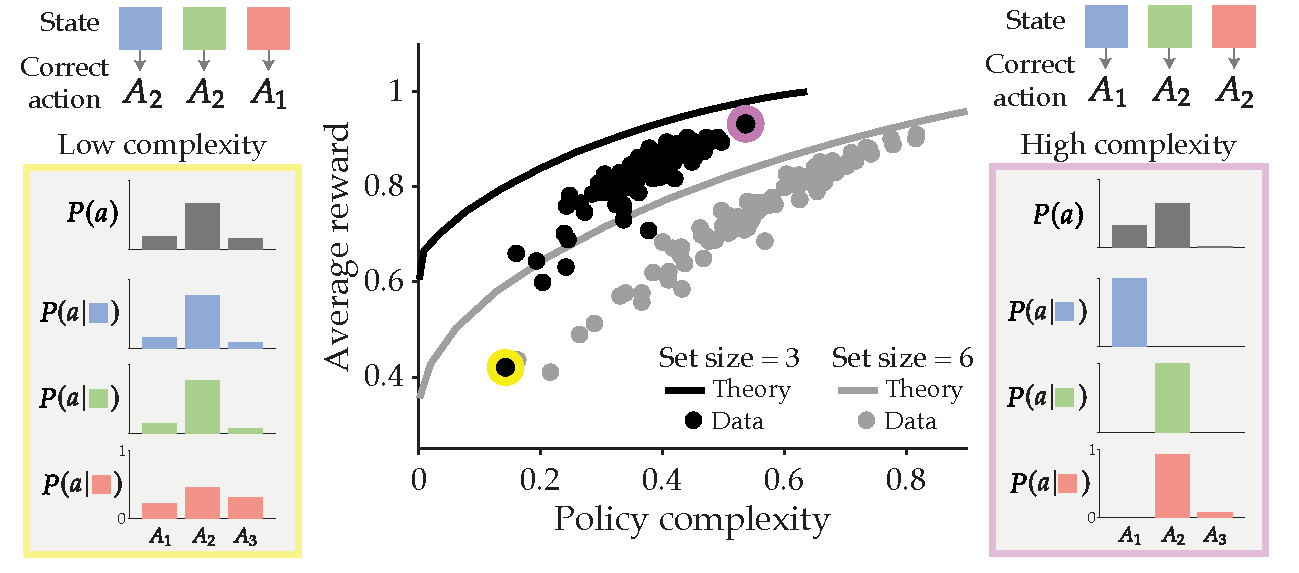
\includegraphics[width=450pt]{figs/gershman20.pdf}
    \caption{\textbf{The reward-complexity trade-off describes the optimal degree of policy perseveration.} Adapted from \cite{gershman20}. (Middle panel) Theoretically optimal reward-complexity trade-off curves (solid lines) for a particular set size (3 or 6). Each data point represents a subject's performance aggregated across blocks of the same set size. (Left panel) Marginal and conditional action probabilities from an example subject (set size = 3) with a low complexity policy. Notice the similarity between the marginal action probability $P(a)$ and the policies conditioned on different states. (Right panel) An example subject with a high complexity policy. Notice the deviation of the state-dependent policies from the marginal action probability.}
    \label{fig:gershman20}
\end{figure}

The tendency to perseverate on past policies, even when inappropriate, is ubiquitous. It has been observed in studies of operant conditioning \citep{thorndike11,lau05}, perceptual decision making \citep{verplanck52,howarth56,frund14}, and choice reaction time \citep{bertelson65}. Perseveration has often been viewed as a kind of irreducible nuisance factor, or as a reflection of habit formation \citep{dickinson85,miller19}. What remains unclear in these accounts is why perseveration should happen at all. Is there a computational logic underlying its existence?

The capacity-limited optimal policy provides one possible answer. Any capacity-limited agent operating at the optimal reward-complexity frontier will exhibit a bias to take actions that have been frequently chosen in the past. This bias comes from the $\log P^\ast(a)$ term in Eq. \ref{eq:optimalpolicy}. The influence of this bias on the overall action policy will depend on the agent's capacity limits, reflected in the value of $\beta$.

\citet{gershman20} argued that policy complexity can be interpreted as an inverse measure of perseveration, because it is higher to the extent that state-specific policies diverge from the marginal policy. When this divergence is low, it means that states exert a weak degree of control over actions, and hence there is a tendency to choose actions with the same probability across all states (see Figure \ref{fig:gershman20}, left panel). Given this interpretation of policy complexity, the empirical reward-complexity trade-off function tells us whether a particular degree of perseveration is optimal given a particular agent's capacity limit. Specifically, we can say that the agent is optimal if their empirical trade-off coincides with the optimal trade-off for a given policy complexity.

\citet{gershman20} estimated the empirical trade-off function using data from a version of the contextual bandit task discussed above \citep{collins18}. Overall, subjects were close to the optimal trade-off curve, though subjects with low policy complexity exhibited a systematic deviation (Figure \ref{fig:gershman20}). This deviation was later explained by \citet{gershmanlai20} as a possible consequence of suboptimal learning: subjects with lower learning rates, as estimated using the actor-critic model presented in the Appendix, showed a greater deviation.

\citet{gershman20} also investigated whether the pattern of perseveration in this data set followed the functional form in Eq. \ref{eq:optimalpolicy}. While it is common for separate coefficients to be estimated for the value and perseveration terms that are entered into the softmax, the optimal policy suggests that only a single coefficient ($\beta$) is necessary. Consistent with this hypothesis, a model with a single coefficient outperformed a model with two coefficients.

Perseveration of policies can often be observed as behavioral inflexibility in response to a change in the environment. For example, consider the widely-used serial reversal learning task, in which selecting one of two stimuli is reinforced while the other is not (Figure \ref{fig:reversal}A). After a subject has learned to consistently choose the reinforced stimulus, the reward contingencies reverse. In this scenario, perseveration would correspond to the inability to adapt choice behavior after reversal. 

\cite{Hassett2017-dv} showed that monkeys trained on this task were slower to adapt to reversals when working memory was taxed by manipulations of cognitive load. This result suggests that working memory is critical for behavioral flexibility as measured by reversal speed, a finding consistent with the idea that perseverative action biases are modulated by capacity limits on memory. This kind of perseveration has also been quantified in rule-switching tasks such as the Wisconsin card sort task \citep{Berg1948-bi} and the dimensional card sort task \citep{Zelazo2006-kj}, where perseveration is not simply a repetition of earlier actions but repetition of an entire policy.

\begin{figure}
    \centering
    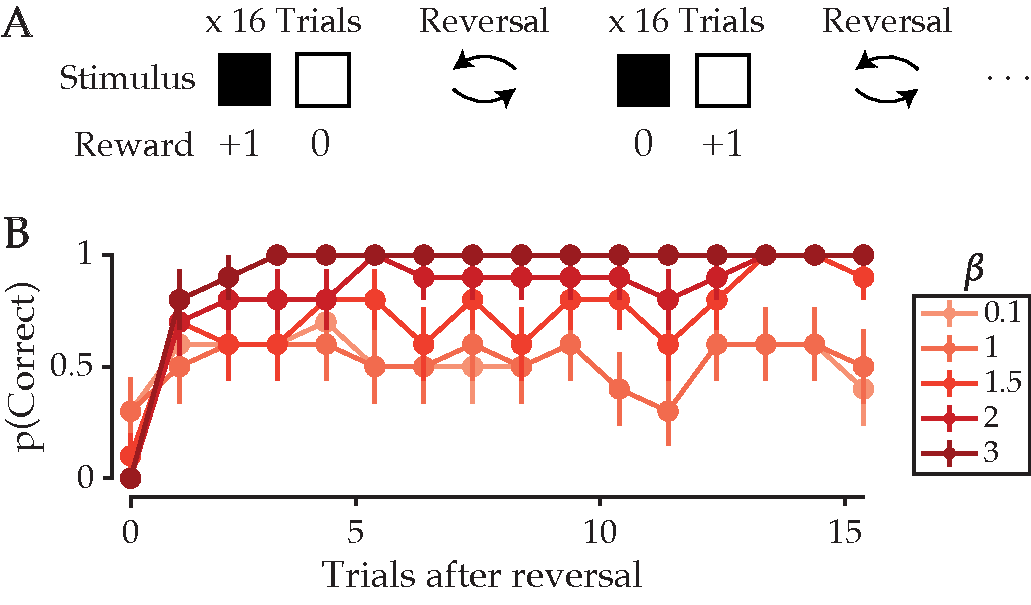
\includegraphics[width=350pt]{figs/reversal.pdf}
    \caption{\textbf{Simulated reversal learning under varying capacity constraints.} (A) In a serial reversal learning task, one stimulus is rewarded while the other is not. After a set number of trials (or when a performance criterion is reached), the reward contingencies reverse. (B) Proportion of trials where the ``correct'' choice was made as a function of the number of trials after reversal. Performance is averaged across 10 reversals. Trial 0 indicates the first trial after the reward contingencies reverse; therefore, agents should still respond according to the contingencies in effect prior to reversal.}
    \label{fig:reversal}
\end{figure}

To explicitly demonstrate the relationship between perseveration and capacity limits on memory, we simulated the performance of five agents with varying capacity constraints on a generic serial reversal learning task (Figure \ref{fig:reversal}A).\footnote{In the rest of the simulations, we specify values of $\beta$ to imply given capacity limits (see Eqs. \ref{eq:optimalpolicy} and \ref{eq:beta}). This allows us to evaluate behavior as a function of capacity under the assumption that $\beta$ implicitly defines a point on the reward-complexity trade-off curve. Alternatively, the value of $\beta$ can be learned from experience. We leave this possibility as an open question for future research.} If behavioral flexibility varies as a function of capacity constraint, we should expect to see faster rule reversals for high capacity agents, and ``stickier'' choice behavior for low capacity agents, indicating the perseverative influence of a previously-learned policy. Indeed, we see that high capacity agents are faster at learning the new reward mapping than low capacity agents, attaining 100\% accuracy just a few trials after reversal has occured (Figure \ref{fig:reversal}B).

Notice that the ``state'' in this task is not the stimulus (as it was in the previous example), but rather, the underlying reward contingencies or context. This again underscores the definition of perseveration as the degree of state-independence of the policy: low capacity agents will not be able to distinguish between different reward contexts and therefore will not perform reversals. At the lowest extreme (e.g., $\beta = 0.1$), agents do not even learn to select the rewarded stimulus due to the strong bias of the marginal action probability (which we assume be uniform across actions at the beginning of learning). This causes an agent to continue responding stochastically (e.g., choosing both stimuli with equal probability) throughout the entire task. As the capacity constraint increases, agents become better able to distinguish between reward contexts, allowing them to detect when the underying state has changed. When the stimulus that was once associated with reward is suddenly no longer rewarded (in Figure \ref{fig:reversal}B, we take this to be Trial 0 after reversal), agents are aware that a state change has occured and reverse their action policy accordingly. 

We have shown that the tendency to perseverate on past policies can be explained by limitations on cognitive capacity: when capacity is low, policies will be biased by the actions taken most often in recent history. When capacity is high, policies will be more sensitive to the current state. Our framework allows us to recast perseveration in the light of an optimal solution under a given capacity limit instead of treating it as a suboptimal behavioral nuisance.

\subsection{Response time}

In a seminal paper, \citet{hick52} studied response times in a task where subjects made speeded responses to one of $N$ possible targets. Hick found that mean response time was an approximately logarithmic function of the number of targets, a regularity now known as \emph{Hick's law} \citep[see][for a recent review]{proctor18}. Hick's law holds not only for target selection (commonly known as \emph{choice reaction time} tasks), but also for the contextual multi-armed bandit task studied by Collins and colleagues \citep{collins12,collins14,collins18}, as shown in Figure \ref{fig:RT}: mean response time is well approximated by a linear function of log set size \citep[see also][for more detailed analyses of response times in this task]{mcdougle20}.

\begin{figure}
    \centering
    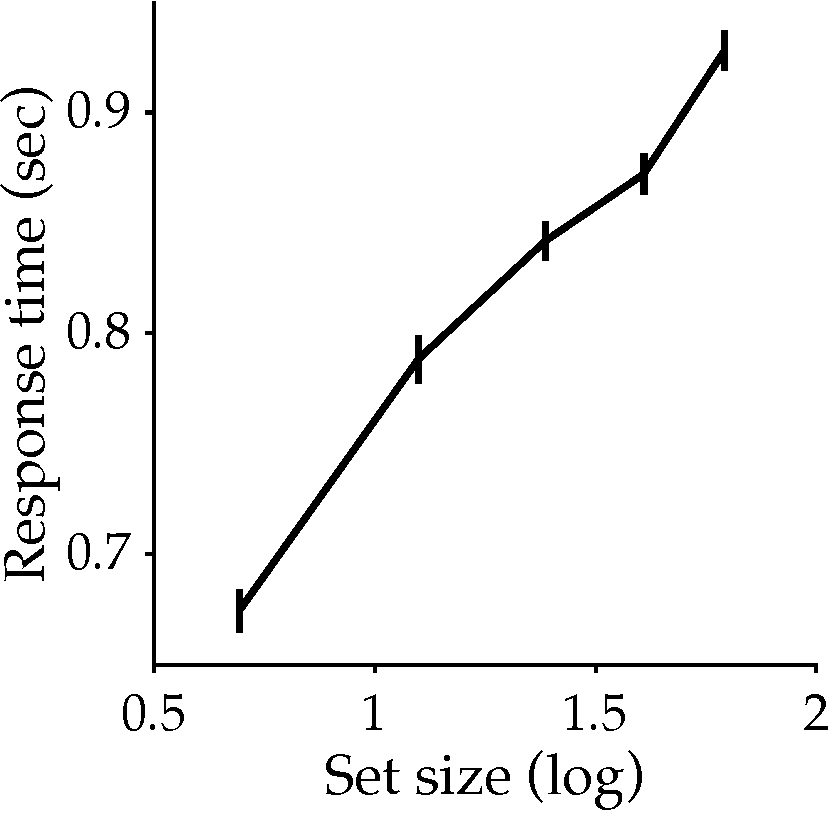
\includegraphics[width=0.35\textwidth]{figs/rt.pdf}
    \caption{\textbf{Average response time as a function of log set size}. Data taken from healthy controls in \citet{collins14} performing the simulus-response task depicted in Figure \ref{fig:stochasticity}A. Error bars show standard error of the mean.}
    \label{fig:RT}
\end{figure}

Hick used an information-theoretic analysis to derive his law. Recall from our discussion of entropy coding that the optimal description length for state $s$ in a noiseless channel is $-\log P(s)$. If each state is equally likely (as in Hick's experiments), then $P(s) = 1/N$ and the optimal description length is $\log N$. In a Huffman code, this corresponds to the number of bits that need to be inspected to reveal the coded state. Thus, if we assume that bits are inspected at a constant rate, we arrive at Hick's law.

More generally, response time should be a linear function of the description length, which can be manipulated even when the number of states is held fixed \citep{hyman53}. Following this logic, we reasoned that people with lower capacity should have longer description lengths (higher policy complexity) and therefore longer response times. Consistent with this prediction, policy complexity was significantly correlated ($r = 0.35, p < 0.0001)$ with mean response time across subjects in the data from \citet{collins18}.

A number of studies have found that the slope of the set size function decreases with practice \citep{hale68,mowbray59,wifall16,teichner74}. One explanation for this finding is that optimal compression depends on knowing the state probabilities, which must be learned. Studies of compression effects in short-term memory have shown that these effects emerge over the course of training \citep{brady09,ngiam19}.

As mentioned earlier, algorithms like Huffman coding seem to require implausibly high precision relative to the level of noise in the brain. This point is relevant to Hick's law, because some studies indicate that the set size function flattens out for very large set sizes, deviating from the law \citep{seibel63,longstreth88}. This would make sense if there is a limit to the number of bits that can be assigned to each codeword, which would constitute a lossy code if the limit is sufficiently low.

A final point about Hick's law, and set size effects more generally, is that these effects are only observed when a policy needs to be retrieved from memory \citep{proctor18}. For example, response time increases with set size if subjects have to move a cursor to target locations indicated symbolically by letters, but not if the target location corresponds to the location of the stimulus \citep{dassonville99}. This observation is broadly consistent with our argument that the memory demand of policies acts as an information bottleneck in action selection.

\subsection{Action chunking}

Imagine you are learning to make coffee. You carefully measure out the beans, grind them in a coffee grinder, put the grounds into your coffee maker, and press a button. Over time, you notice that you get faster and faster at making coffee, and eventually, it requires little thought or attention---you could do it with your eyes closed. This example illustrates the idea that learned sequences of actions eventually become automatic and quick to execute.

Many skills in our everyday lives, such as making coffee, are learned by repeatedly sequencing actions in the service of a desired goal. The action sequence can become automatic such that once started, it must be brought to completion. These observations underlie the defining characteristics of action ``chunks''---the reflexive association of a number of independently produced actions into rapidly executed action sequences \citep{dezfouli12,lashley51,sakai03,botvinick08}.

Examples of action chunking are ubiquitous, especially in the sequence learning literature \citep{Terrace1991-di,Verwey1999-fn,sakai03,Miyapuram2006-gb}. Animals show evidence of action chunking in the formation of habitual action sequences \citep{Graybiel1998-sw,jin10,jin14}. In the machine learning literature, action chunking is closely related to ``options'' \citep{Precup1998-wo,Precup2000-qa}, or temporally extended action sequences that allow agents to plan more efficiently and accurately. 

In an important paper on sequence learning, \cite{sakai03} showed that human subjects can learn a visuomotor sequence by spontaneously chunking elementary movements together, where each chunk acts as a single action unit. They showed that execution time decreased as a function of sequence repetition during learning. To test for the formation of chunks, they shuffled the visuomotor sequences and found that the performance on a shuffled sequence was both faster and more accurate when the action chunks in the original sequence were preserved (within the shuffled arrangement) compared to when they were destroyed.  These results are also consistent with evidence that people reuse learned action chunks, even when the chunks are suboptimal for the task at hand \citep{Huys2015-cq}. 

Action chunks are advantageous because they allow for the production of rapid action sequences without having to rely on the selection of individual elements. In this view, an action chunk can be treated as a single response such that selecting a familiar movement pattern only involves a single processing step. It has been suggested that the formation and expression of action chunks provides a mechanism for the execution of action repertoires that would otherwise be too biologically costly to implement \citep{graybiel98,ramkumar16}. In this way, chunks reduce the amount of memory necessary to execute a sequence of actions by effectively compressing state information. Consistent with this idea, some studies have demonstrated a relationship between spatial working memory capacity and the learning of new action chunks \citep{Bo2009-pa, Seidler2012-ab}.

Why might action chunks cost less from an information processing perspective? Recall that the complexity of an action policy depends on the degree to which it is state-dependent. In other words, we can think of policy complexity as quantifying the amount of memory that must be devoted to the state information when selecting actions. When the sequence of actions involved in making coffee becomes an action chunk, there is no longer a need to pay close attention to the ``states'' associated with each action (e.g., the particular brand of coffee beans being used, the grinder setting, and particular coffee maker). Furthermore, this sequence of actions would be the same regardless of whether you were making coffee at home or at your friend's home (assuming that you aren't particularly picky about your choice of coffee beans). Every morning, this familiar sequence is initiated by the first action of picking up your bag of coffee beans, and brought to completion without needing to process state information beyond noting where the coffee beans are stored.

In the following example, we show that multi-step action sequences are preferred when there is an imperative to reduce policy complexity. Specifically, as capacity is reduced, the preference for multi-step action chunks should increase, while the action execution time should decrease. This is because for low complexity agents, it is more cost- and time-effective to select an action chunk of length $n$ than it is to select $n$ independent actions.

Imagine a task environment in which every state cues a specific rewarded action (Figure \ref{fig:ac1}A). States appear in sequence, and an agent's task is to select the correct action as quickly as possible.\footnote{This is similar to many tasks used to study motor skill learning, for example, the Discrete Sequence Production task \citep{Verwey1999-fn} or the Serial Reaction Time Task \citep{Nissen1987-vn,Robertson2007-pv}.} Agents can select from five different actions: four ``independent'' ones, as well as one action ``chunk'' (Figure \ref{fig:ac1}B).\footnote{We include only one possible action chunk in this example for simplicity, though we recognize that any combination of actions of any length could also be considered an action chunk. We also do not address how these chunks are learned, and leave that as an open question for future research.} Following previous work suggesting that an action chunk acts as a single action unit \citep{graybiel98,sakai03}, we also assume that it takes an equal amount of time to execute an independent action as it does to execute an action chunk. If a chunk of length $n$ is selected on trial $t$, the actions in the chunk set will be executed until $t+n-1$ (instead of using the policy to select actions). In our process model (as described in the Appendix), selecting an action chunk will inherently cost less because the agent does not need to factor in policy costs from time $t+1$ to $t+n-1$. This effectively means that agents can ignore all incoming state information until they are finished executing the action sequence. 


\begin{figure}
    \centering
    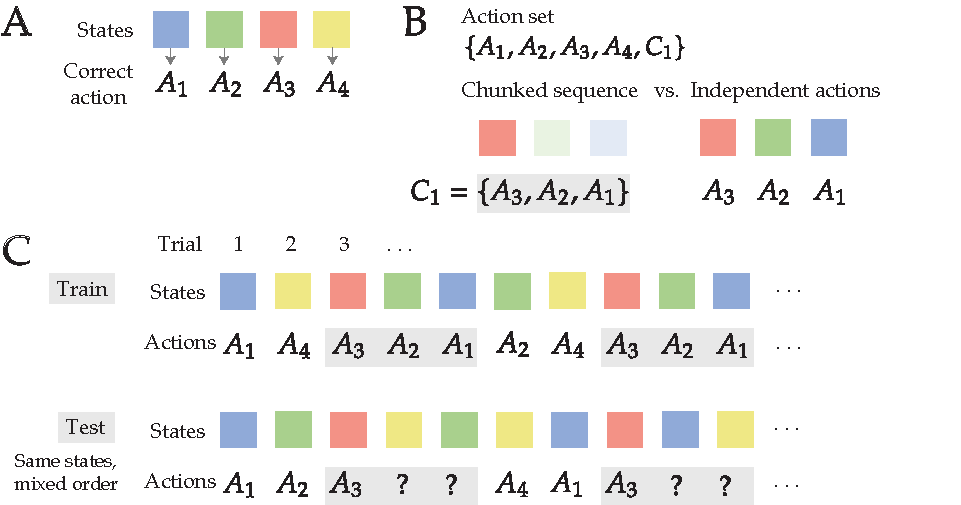
\includegraphics[width=0.9\textwidth]{figs/ac1.pdf}
    \caption{\textbf{A generic action chunking task.} (A) A stimulus-response task with four states and four corresponding actions. Selecting the correct action in each state leads to a reward of +1. (B) The valid action set. For simplicity, imagine that agents can either select independent actions ($A_1, A_2, A_3, A_4$), or select the action chunk $C_1$, which is composed of the action sequence: $\{A_3,A_2,A_1\}$. Notice that for the same three state sequence (red, green, blue), selecting three correct independent actions will lead to the same total reward (3) as if the action chunk was selected. However, in selecting the action chunk, agents no longer have to pay attention to the states following the chunk-initiating state (red). (C) Agents first learn the correct state-action pairings in a ``Train'' block. The task is designed such that a specific state sequence (red, green, blue) reoccurs often. Over the course of training, agents should recognize this state sequence and choose to select the action chunk $C_1$ in the red state instead of taking independent actions in each of the states occuring in sequence. In the ``Test'' block, agents are exposed to the same states as seen in the ``Train'' block, but in randomized order. Now that the reoccuring state sequence is eliminated, one can measure the degree of chunking learned in the ``Train'' block by observing the actions taken in the two states following the original chunk-initating state.}
    \label{fig:ac1}
\end{figure}

If the task environment consists of predictable temporal relationships across states (e.g., if a certain sequence of states occurs over and over again), agents will naturally begin to select the same sequence of actions in response to this state sequence. In our specific example, agents frequently observe the same three state sequence (red, green, blue) within the ``Train'' block of the task (Figure \ref{fig:ac1}C). Later, in a ``Test'' block inspired by the task in \cite{sakai03}, this three state sequence is destroyed by shuffling the order in which states appear. This manipulation provides a way to observe how the reuse of learned action chunks when they are no longer advantageous varies as a function of the agent's memory capacity.

Agents can either choose to select actions upon presentation of each state (``independent'' selection of $A_3,A_2,A_1$), or can choose to select the action chunk that consists of three actions in sequence, $C_1 = \{A_3,A_2,A_1\}$. While these two action plans lead to the same total reward (3), selecting the action chunk frees agents from having to pay attention to the states following the chunk-initiating state (red). As noted previously, this reduces policy costs, since the agent can ignore some state information. Since there are fewer states to decode information from, the action sequence is also produced more quickly.

\begin{figure}
    \centering
    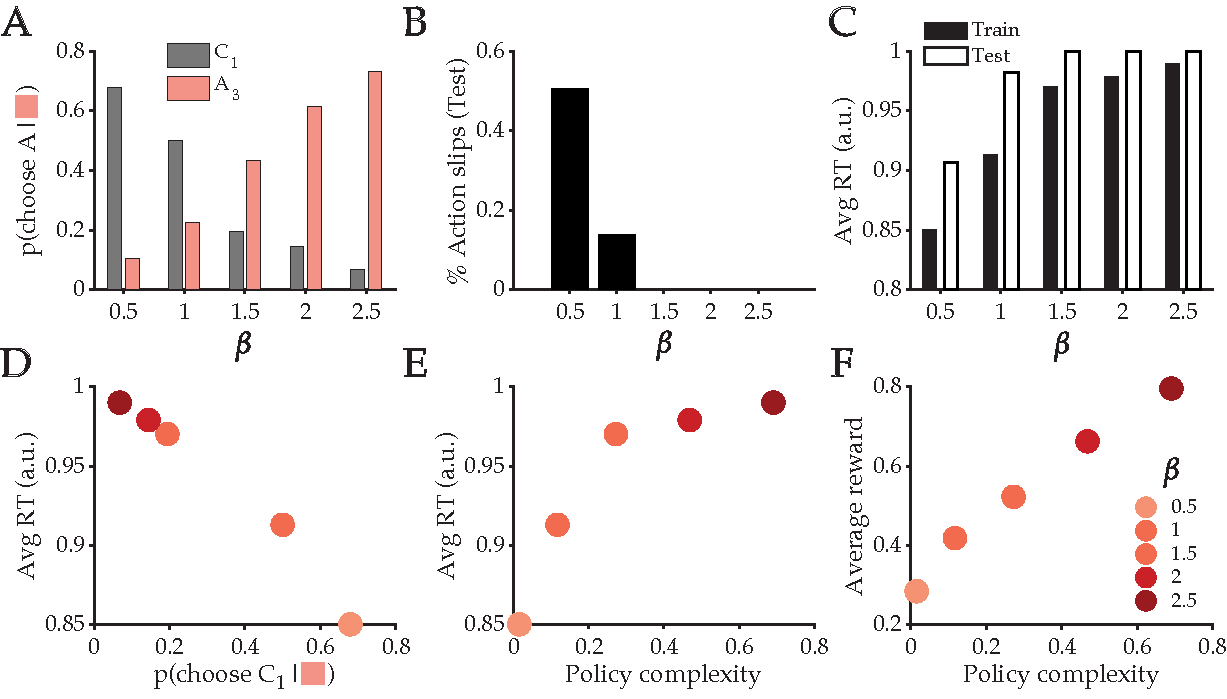
\includegraphics[width=\textwidth]{figs/ac2.pdf}
    \caption{\textbf{Action chunking under resource constraints.} (A) Proportion of trials where $A_3$ or $C_1$ was chosen in the red state (see Figure \ref{fig:ac1}). (B) The percentage of ``action slips'' in the ``Test'' block (quantified as choosing $C_1$ in the red state when it is no longer the optimal action) as a function of capacity, $\beta$. (C) Average response time (RT) per trial as a function of capacity. (D) Average RT as a function of the proportion of trials where $C_1$ was chosen in the red state. (E) Average RT as a function of the policy complexity. (F) The reward-complexity trade-off for different capacities.}
    \label{fig:ac2}
\end{figure}

In Figure \ref{fig:ac2}A, we show that the preference for selecting multi-step action chunks $C_1$ in the chunk-initiating red state decreases as a function of the capacity. This is consistent with the intuition that low capacity agents should prefer chunked action sequences because they compress information, while high capacity agents can afford to retain more state information (and therefore take state-specific actions). As stated earlier, one consequence of learning a preference for action chunks is that they are often reused even when this is suboptimal \citep{Huys2015-cq}. To show this, we counted the number of  ``action slips'' \citep[cf.][]{norman81}, defined as the percentage of trials where the action chunk $C_1$ was taken in the chunk-initiating state when it was no longer optimal, and saw that it was higher at lower capacity constraints. 

Additionally, we confirmed that the average response time per trial increased in the ``Test'' block across all capacity constraints (but especially for lower-capacity agents), reflecting the increase in processing time necessary when chunks are no longer being used. This means that the average response time overall should decrease as a function of the proportion of trials where the action chunk was selected (Figure \ref{fig:ac2}D). In analog to Figure \ref{fig:RT}, we also observe the RT increasing as a function of policy complexity (Figure \ref{fig:ac2}E), consistent with the information-theoretic analysis of Hick's Law.


\subsection{State chunking}

Real-world environments contain a large number of states, and the brain's capacity limit means that it is typically not efficient to represent all states with the same fidelity. Especially in environments where states are correlated (e.g., if they lead to the same reward or policy), it can be advantageous and cost-effective to merge similar states into state ``chunks.''

State chunking confers several advantages. By generalizing across similar states, information learned in one state can be efficiently re-used and transferred across other states that share similar reward and transition structures \citep{Abel2019-hr,Lehnert2019-kz,tomov20,Lehnert2020-nv}. Recent work has suggested that for long-term benefits, agents should focus on learning reward-predictive state abstractions \citep{Lehnert2019-kz,Lehnert2020-nv}, implying that if states share common futures, then they will become chunked together. However, there are also situations in which generalization may not be advantageous. For example, if the reward structure of an environment suddenly changes in a manner that is not supported by the learned state chunk, an agent will lose out on reward if it continues to follow the same policy. 

\begin{figure}
    \centering
    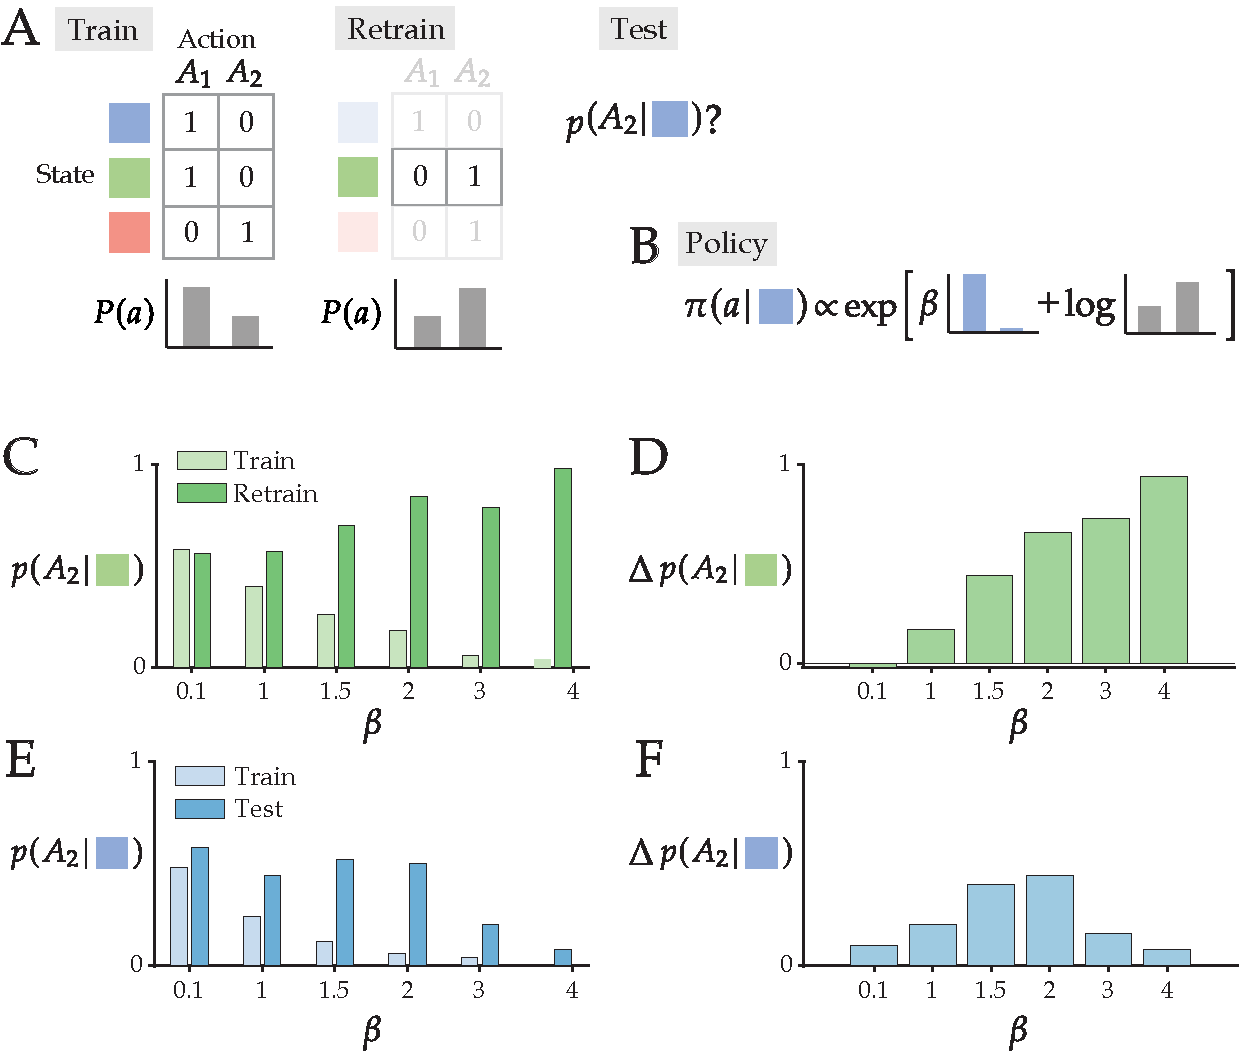
\includegraphics[width=0.9\textwidth]{figs/sc.pdf}
            \caption{\textbf{State chunking under resource constraints.} (A) Consider a task with three distinct states (blue, green, and red) and two actions ($A_1$ and $A_2$). In the ``Train'' block, agents learn that taking action $A_1$ in the blue and green states and action $A_2$ in the red state leads to reward. After training, the marginal probability P(a) is biased towards $A_1$. In the ``Retrain'' block, agents learn a new reward mapping for the green state---now, taking action $A_2$ in the green state is rewarded. After retraining, the marginal probability P(a) is now biased towards $A_2$. To quantify the amount of state chunking, we introduce a ``Test'' block where we measure the proportion of trials where an agent choses action $A_2$ in the blue state. (B) A graphical depiction of the policy, decomposed into the state-action values and the marginal action probability. The relative influence of each component on action selection will depend on the value of $\beta$. (C) The proportion of choosing $A_2$ in the green state as a function of the capacity constraint for the ``Train'' and ``Retrain'' blocks. (D) The change in proportion of trials where $A_2$ is chosen in the green state as a function of capacity constraint ($\Delta p = $ Retrain - Train). (E) The proportion of choosing $A_2$ in the blue state as a function of the capacity constraint for the ``Train'' and ``Test'' blocks. (F) The change in proportion of trials where $A_2$ is chosen in the blue state as a function of the capacity constraint ($\Delta p = $ Test - Train).}
    \label{fig:sc1}
\end{figure}

In the following example, we will demonstrate that state chunking arises under the imperative to compress policies. Specifically, we will show that lower capacity agents are more likely to chunk states leading to similar reward, but are also less likely to adapt to changes in the reward environment. In contrast, higher capacity agents are able to flexibly and quickly adapt to changes in the environment in a state-specific manner.

Consider a task environment with three distinct states (blue, green, and red) and two actions ($A_1$ and $A_2$; Figure \ref{fig:sc1}A). In the ``Train'' block, agents learn that taking action $A_1$ in the blue and green states and action $A_2$ in the red state leads to reward. Note that after training, the marginal probability $P(a)$ is biased towards $A_1$. In the ``Retrain'' block, agents learn a new reward mapping for the green state---now, taking action $A_2$ in the green state is rewarded. After retraining, the marginal probability $P(a)$ is now biased towards $A_2$. To quantify the amount of state chunking, we introduce a ``Test'' block where we measure the proportion of trials where an agent choses action $A_2$ in the blue state. 

Figure \ref{fig:sc1}B depicts the relative contribution of the state-action values and the marginal action probability to the final policy. Critically, action selection in the ``Test'' block will depend on the agent's given capacity limit as stipulated by $\beta$. If there is no need for compression ($\beta$ is high), then the agent should respond to the blue state exactly as it did in the ``Train'' block. However, if the capacity constraint is low and there is a need to compress information ($\beta$ is low), agents will end up relying on the marginal action probability, which allows them to ignore some state information. This means that the proportion of choosing action $A_2$ in the blue state in ``Test'' will be greater than in the ``Train'' block. 

We will first examine learning in the ``Retrain'' block. Figure \ref{fig:sc1}C shows the probability of choosing $A_2$ in the green state as a function of the capacity constraint ($\beta$). Note that agents with higher capacity constraints are better at adapting to the new reward structure in the ``Retrain'' block, choosing $A_2$ more often than in the ``Train'' block. Figure \ref{fig:sc1}D shows that the change in proportion of trials where $A_2$ is taken is increasing as a function of capacity constraint, indicating a greater ability to adapt to the new reward structure at higher capacity constraints.

To understand how capacity constraints affect the chunking of the blue and green states, we can examine choice behavior in the ``Test'' block. As mentioned previously, if the blue and green states were chunked together in the ``Train'' block, we should see an increase in the probability of choosing $A_2$ in the blue state from ``Train” to ``Test'' blocks. Figure \ref{fig:sc1}E shows that the probability of choosing $A_2$ decreases as a function of the capacity constraint in the ``Train'' block, and remains roughly constant before decreasing in the ``Test'' block.

A nuanced result is shown in Figure \ref{fig:sc1}F, where we show that the change in proportion of trials where $A_2$ is chosen is increasing and then decreasing as a function of capacity constraint. To understand this nuance, consider the lowest capacity agent ($\beta = 0.1$), who selects actions based on their marginal action probability $P(a)$, assumed to be uniform across actions at the beginning of learning. As a result, responding remains stochastic throughout both ``Train'' and ``Test'' blocks, so there is no significant change between the probability of choosing $A_2$ in the blue state across blocks. However, for intermediate capacity constraints, the policy is influenced by both the state-action values and the marginal action probability (Figure \ref{fig:sc1}B). As capacity increases ($\beta = 1, 1.5, 2$), the marginal action probability $P(a)$ will become more peaked and influence the policy in the blue state, causing the agent to choose $A_2$ more frequently in ``Test'' relative to ``Train.'' But as capacity continues increasing ($\beta  = 3, 4$), the probability of choosing $A_2$ begins decreasing, because now the state-action values learned in ``Train'' alone should dominate the policy.

These results demonstrate that state chunking can arise out of a need to compress state information by merging states that lead to the same reward when there are limits on capacity. At one extreme, low capacity agents do not learn much at all, and their responding remains stochastic. At the other extreme, high capacity agents can perfectly learn and store state-dependent policies, and flexibly adapt to new reward structures. Between the two extremes, there is a dynamic range of behavior that varies depending on how much state-specific action information an agent can afford to store in memory.

 \subsection{Navigation}
 
Navigation is a form of goal-directed behavior that requires an organism to plan complex sequences of actions towards a desired location. Maze tasks such as the Morris Water Maze, radial arm maze, and T-maze have been used in the animal learning literature to study navigation, and behavioral performance is typically measured by the amount of time it takes subjects to reach a goal location. However, this performance criterion ignores the complexity cost of a particular action trajectory, which is related to how \textit{state-specific} a trajectory is.

To illustrate this, imagine that you have the choice of driving to two grocery stores, one that is closer and one that is farther away. While driving time alone might suggest that the closer store is preferred, it may not take into account the fact that driving to the closer store requires you to turn at a number of intersections (high policy complexity), while driving to the store that is farther away would only require staying on a highway for most of the trip (low policy complexity). The former route requires you to remember more about the specifics of your current location (or state) in order to successfully navigate to your final destination, while the latter does not. This example highlights the fact that the state-specificity of a navigational policy incurs a computational cost that must be taken into account by behaving agents.

In a recent study, \cite{Amir2020-lm} used the reward-complexity trade-off to analyze the learning processes of mice navigating to a hidden platform in the Morris Water Maze task. Specifically, they quantified the trade-off between the value and complexity of an animal's swimming trajectories across four days of learning. The value of a swimming trajectory was related to its energy cost and was correlated with swimming time, while the complexity of a trajectory provided a measure of the computational cost needed to generate specific, goal-directed motor plans at any given location. Complexity was measured relative to the swimming trajectories of naive animals, which by definition had the lowest policy complexities. Trained animals exhibited swimming trajectories that were often shorter and more direct, which increased the value of the trajectory but also incurred a higher complexity cost. This increased cost reflects the fact that trained animals took into account their current location or state on a moment-by-moment basis in order to orient their swimming direction towards the goal platform.

Animals tended to optimize for value early in learning while reducing policy complexity later in learning (by finding less costly trajectories that maintained the same value). This corresponds to movement \textit{along} the optimal reward-complexity curve over the course of training. To summarize the learning state of an animal at a given time, \cite{Amir2020-lm} fit values of $\beta$ to the data from each day and found that it increased over the four days of learning.\footnote{In our simulations, we have chosen to assume a fixed value of $\beta$ for simplicity. But as this study suggests, $\beta$ is likely to evolve over the course of learning as agents move along the optimal reward-complexity frontier. Future work should investigate how $\beta$ can be learned depending on the optimal policies and reward statistics unique to particular task environments.} The trade-off between value and complexity effectively captured the behavioral dynamics of navigational learning: as mice gained more details about the location of the goal platform, they increased the precision of their motor commands and were able to quickly swim towards the platform from any starting location in the tank. 

\subsection{Psychiatry}

What happens when humans fail to optimize the reward-complexity trade-off? As mentioned previously, the incremental nature of our proposed learning algorithm (see Appendix) means that it will spend a non-trivial amount of time away from the optimal reward-complexity trade-off curve. In fact, as long as learning is incomplete, agents will exhibit suboptimality. This suboptimality in learning offers one potential explanation for the maladaptive behaviors observed in many psychiatric conditions (e.g., schizophrenia, OCD, Tourette's, Parkinson's disease). While we recognize that there could be various explanations for the behavioral deficits observed in these conditions, we focus primarily on the influence of deficits in working memory capacity on behavior. 

\begin{figure}
    \centering
    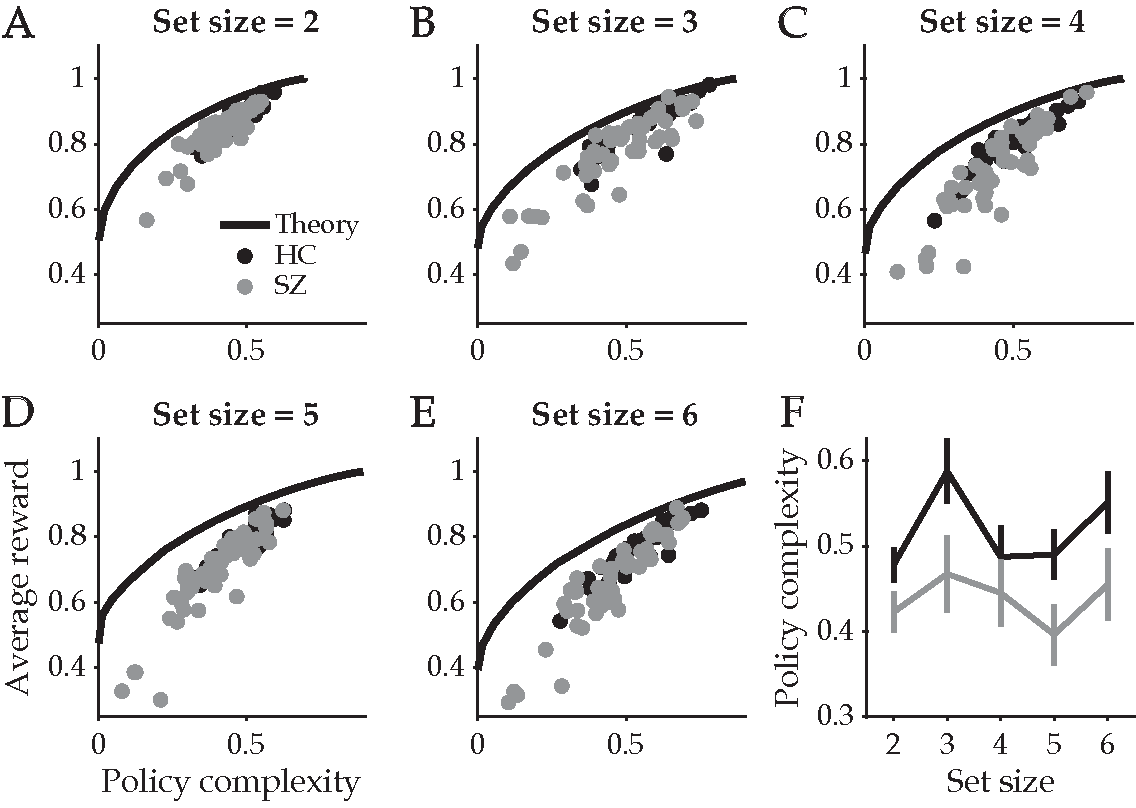
\includegraphics[width=0.9\textwidth]{figs/collins14main.pdf}
            \caption{\textbf{The reward-complexity trade-off for schizophrenia patients and healthy controls.} Adapted from \cite{gershmanlai20}, data from \cite{collins14}. The optimal reward complexity curves (solid lines) for each given set size (2 to 6). Solid circles are the empirical reward-complexity values for each subject (HC = healthy controls; SZ = schizophrenia patients). (B) Policy complexity as a function of set size. Error bars show 95\% confidence intervals.}
    \label{fig:collins14main}
\end{figure}

Working memory and cognitive effort deficits are a well-known characteristic of schizophrenia \citep{culbreth18,forbes09}. It therefore stands to reason that these patients should exhibit pronounced sub-optimality in their reward-complexity trade-off. To pursue this question, \cite{gershmanlai20} compared the performance of patients to healthy controls in the Collins contextual bandit task depicted in Figure \ref{fig:stochasticity}. Figure \ref{fig:collins14main} shows the optimal and empirical reward-complexity trade-offs, as well as the average policy complexity across patients and healthy controls for tasks of varying set sizes, demonstrating that patients had systematically lower policy complexity but appeared to lie along the same empirical reward-complexity trade-off curve as healthy controls. Additionally, Gershman and Lai showed that empirical deviations from the optimal curve (``bias'') in both populations increased as a function of set size and decreased as a function of policy complexity (Figure \ref{fig:collins14bias}). This pattern of bias could be explained as a consequence of suboptimal learning, as reflected in the lower learning rates of schizophrenic patients as compared to healthy controls. 

\begin{figure}
    \centering
    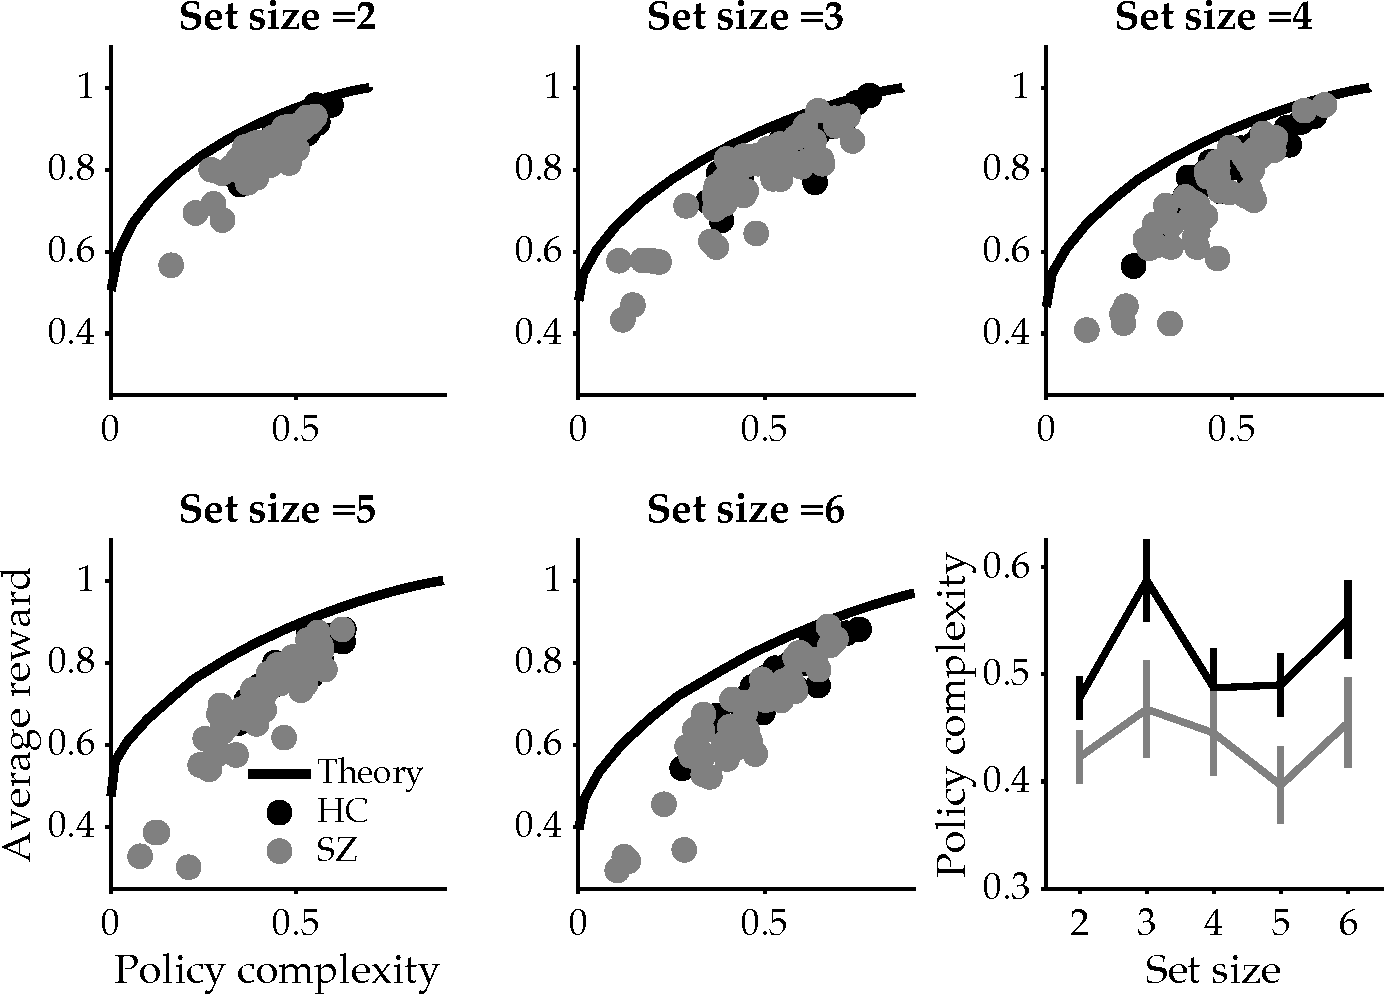
\includegraphics[width=0.9\textwidth]{figs/collins14bias.pdf}
            \caption{\textbf{Bias in schizophrenic patients and healthy controls.} Adapted from \cite{gershmanlai20}, using data from \citet{collins14}. (A) Bias, or the deviation of the empirical from the optimal reward-complexity curves, as a function of set size for the schizophrenia (SZ) and healthy control (HC) groups. Error bars show 95\% confidence intervals. (B) Bias as a function of policy complexity.}
    \label{fig:collins14bias}
\end{figure}

In probabalistic reversal learning tasks, schizophrenic patients have been shown to achieve fewer reversals than controls as well as decreased win-stay/lose-shift behavior. Patients also do not see errors as being informative of a context shift, suggesting some insensitivity to the underlying reward state \citep{Culbreth2016-rs,Schlagenhauf2014-oz}. One large study of probabalistic reversal learning in schizophrenia found that patients exhibit more suboptimal behavior as compared to healthy controls \citep{Reddy2016-ew}. Specifically, schizophrenic patients had a higher proportion of lose-stay (selecting the same stimulus when it was previously unrewarded) and win-shift (selecting an alternate stimulus when the previous stimulus was rewarded) behaviors than did healthy controls. 

Could it be that schizophrenia patients have overall lower capacity limits, which affect learning in cognitive tasks? To explore this possibility, we used the same reversal learning simulation in Figure \ref{fig:reversal} to show that the need to compress policies can lead to suboptimal behaviors in reversal strategy. In Figure \ref{fig:revsz}, we show that as capacity is reduced, the proportion of lose-stay and win-shift behaviors increases, a result consistent with data from schizophrenic patients \citep{Reddy2016-ew}.

\begin{figure}
    \centering
    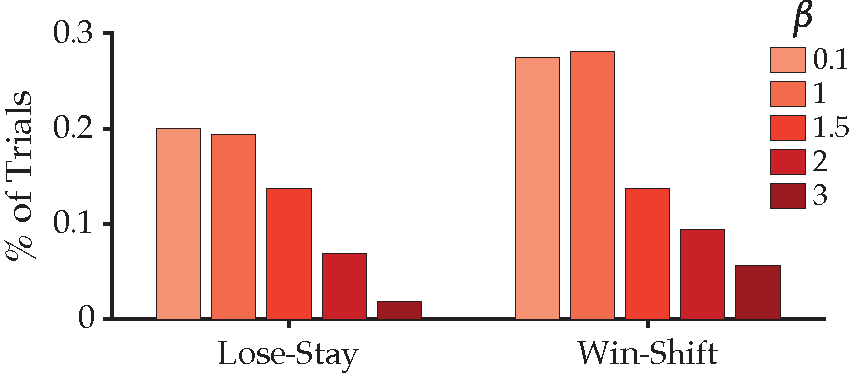
\includegraphics[width=0.6\textwidth]{figs/revsz.pdf}
            \caption{\textbf{Suboptimalities in reversal learning.} The proportion of trials where agents exhibited lose-stay (selecting the same stimulus when it was previously unrewarded) and win-shift (selecting an alternate stimulus when the previous stimulus was rewarded) behavior as a function of different capacity constraints. When the capacity limit is reduced, the proportion of both suboptimal strategies increases.}
    \label{fig:revsz}
\end{figure}

The computational phenotyping of psychiatric illness is still in its infancy. However, the trade-off framework offered here provides a way to evaluate systematic suboptimalities in behavior resulting from deficits in memory capacity. While we have only focused here on the behavioral deficits observed in schizophrenia, these principles could be applied to other psychiatric conditions as well.


\section{Neural signatures of policy compression}

Now that we have seen all the ways in which action selection is shaped by constraints on memory capacity, it seems reasonable to ask: How do neurons in the brain learn the appropriate degree of policy compression? Some answers may be found in our cost-sensitive actor-critic model, which learns the appropriate policy complexity given a biological agent's resource constraints (see Appendix for more details). From an anatomical perspective, our model suggests a computational rationale for the massive compression factor in the mapping from cortex to striatum---if most incoming state information can be disregarded when selecting actions, the basal ganglia can afford to compress incoming cortical information \citep{Bar-Gad2003-fn}. 

From a mechanistic learning perspective, our model implements compression by incrementally modifying the policy based on reward feedback, with the critical assumption that an agent is penalized for policies that deviate from the marginal action distribution. This penalty enters into the reward prediction error (RPE), which in turn affects the policies that an agent will learn. This has direct biological implications: if learning is sensitive to the desire to compress policies, we should see the RPE signal, thought to be communicated by phasic dopamine, vary as a function of a subject's policy complexity. 

While there have not yet been any experimental studies directly investigating the relationship between dopaminergic RPE and policy complexity, several studies from the action chunking literature have hinted at possible downstream effects within the striatum that reflect a neural signature of policy compression. Some have suggested that the ``recoding'' within the striatum seen during stimulus-response learning is responsible for chunking the representations of action sequences so that they can be implemented as single performance units \citep{graybiel98}. Moreover, the learning of action chunks is often reflected in the emergence of ``start/stop'' activity within the striatum that brackets the beginning and end of learned sequences, as well as neural activity that is sustained throughout the execution of an entire sequence \citep{Graybiel1998-sw,Smith2013-ji,jin10,jin14}. This reorganization of neural activity could be one implementation of compression: the ``start/stop'' activity indicates when a subject's attention must be given to the state (namely, at the start and termination of an action chunk), while the sustained activity reflects the fact that an action sequence currently in execution is impervious to the environmental state (and therefore, the neural activity is the same across states). This kind of neural activity would reflect a measure of policy complexity by signaling the moment-by-moment state-dependence of an animal's actions. Similar sensitivity for learned behavioral sequences has been observed in parts of the lateral and dorsomedial prefrontal cortices, with the latter shown to be necessary for the formation of action chunks \citep{Shima2007-ps,ostlund09}. 

Beyond the downstream effects of phasic dopamine, others have suggested that tonic dopamine levels may act as a pseudo-temperature signal by directly modulating striatal excitability and thus tuning the trade-off between reward and policy complexity \citep{parush11}. If tonic dopamine is a neural correlate of the $\beta$ parameter described in our framework, it should reflect a subject's capacity constraint and predict various  behavioral measures of compression as detailed in this chapter. For example, \citet{rutledge09} found that perseveration increases in Parkinson's disease and decreases with dopamine therapy. This result is actually opposite what is predicted by the model in \citet{parush11}, but nonetheless indicates that tonic dopamine plays a role in governing perseveration.

\section{Compression and learning}

In communication systems, compression is a solution to the problem of limited capacity---the overflow of data, so to speak. But in learning systems, compression is a solution to the problem of limited experience---the underflow of data. In order to generalize effectively from finite data, it is necessary to have an inductive bias favoring some generalizations over others. Otherwise, an unlimited number of generalizations are equally plausible given a finite data set. In statistical machine learning, inductive biases that provide generalization guarantees have been formalized under different assumptions and learning objectives. It turns out that a number of these generalization guarantees can be understood as statements that ``compression implies learning'' \citep{blum03,blumer87}.

To get a feel for why this is true, consider an agent that receives a stream of state-action-reward samples. The agent learns a policy from these ``training'' samples, and the question then is whether this policy will generalize effectively to new ``test'' samples. That is, will following the learned policy yield high reward? If the policy is complex enough, then it will favor actions that yield high reward on the training samples, but a policy that is too complex can also fit noise in the data, and hence \emph{overfit}, yielding low reward on the test samples. Thus, policies that balance reward and complexity are more likely to generalize.

The link between compression and learning has been examined from a different angle by recent work on the nature of multitasking constraints \citep{musslick17,musslick20,sagiv18}. The motivating puzzle is why, given billions of neurons, the brain suffers from an inability to simultaneously perform certain tasks at the same time? The basic answer is that even a relatively small amount of overlap in neural pathways can produce a catastrophic degree of cross-talk \citep{feng14}. This begs the question why the brain is evolved to be so susceptible to cross-talk. The answer proposed by Musslick and colleagues is that the upside of pathway overlap is efficiency of learning: shared representations facilitate generalization by reducing the number of separate parameters that need to be learned across tasks (or states). This recapitulates the point that compression (in this case, sharing of representations) is necessary for effective generalization. To mitigate the deleterious effects of cross-talk on task performance, the brain has an additional mechanism, cognitive control, which acts to selectively and strategically potentiate specific representations.

\section{Conclusion}

We have argued that the trade-off between reward and complexity is a fundamental optimality principle in action selection with broad empirical implications. Seemingly unrelated phenomena (perseveration, stochasticity, response time, state and action chunking, and navigation) are woven coherently together within this framework. A unifying theme is that memory limitations play an important role in governing action selection. In this sense, our framework intersects with recent work using rate-distortion theory to understand human memory \citep{bates19,bates20,sims12,sims16,nagy20}. This intersection suggests that we can continue to derive new insights into action selection by drawing parallels with other capacity-limited memory systems.

\subsection*{Acknowledgements}

We are grateful to Dan McNamee for helpful comments. This research was supported by the Center for Brains, Minds, and Machines (funded by NSF STC award CCF-1231216) and a Graduate Research Fellowship from the NSF.

\bibliographystyle{apalike}
\bibliography{bib}

\newpage

\section*{Appendix}

In this section, we derive a generalization of the process model presented in \citet{gershmanlai20}. Code used to reproduce the simulations is available at \url{http://github.com/lucylai96/plm/}.

The optimization problem facing an agent is to maximize expected reward subject to the constraint that the policy complexity (information rate) cannot exceed the agent's capacity $C$. Expected reward under policy $\pi$ is defined as follows:
\begin{align} 
V^\pi= \sum_{s}P(s)\sum_{a}\pi(a|s)Q(s,a),
\end{align}
where $P(s)$ is the probability of state $s$ and $Q(s,a)$ is the expected reward in state $s$ after taking action $a$.

To solve the constrained optimization problem, we write it in Lagrangian form, with Lagrange multipliers $\beta$ and $\lambda(s)$:
\begin{align}\label{eq:5}
    \pi^\ast = \argmax_{\pi} \beta V^\pi - I^{\pi}(S; A) + \sum_s \lambda(s) \left( \sum_a \pi(a|s) -1 \right).
\end{align}
The optimal policy $\pi^\ast$ has the form stated in Eq. \ref{eq:optimalpolicy}. The question we address here is how to tractably find the optimal policy.

We can cast the optimization problem in a form amenable to reinforcement learning by rewriting the Lagrangian as follows (leaving the non-negativity and summation constraints on $\pi$ implicit):
\begin{align}
\pi^\ast = \argmax_\pi \mathbb{E}\left[\beta r - \log \frac{\pi(a|s)}{P(a)}\right],
\label{eq:objfun}
\end{align}
By taking the gradient of the objective function with respect to the policy parameters and using it to incrementally modify the policy, we obtain a ``policy gradient'' algorithm \citep{sutton18} that will converge to the optimal policy. The algorithm takes the form of an ``actor-critic'' architecture consisting of a paramtrized policy (the actor) and a value estimator (the critic). Critically, this algorithm does not require marginalizing over the state space, as in the Blahut-Arimoto algorithm.

Following the functional form of the optimal policy (Eq. \ref{eq:optimalpolicy}), we parametrize the ``actor'' component of the model according to:
\begin{align}
\pi_\theta(a|s) \propto \exp \left[ \beta \theta_a \cdot \phi(s) + \log P(a) \right],
\end{align}
where $\theta$ denotes the adjustable policy parameters and $\phi(s)$ denotes a set of state features. These features will vary across task domains. Taking the gradient of the objective function with respect to $\theta$ yields the following learning rule after taking action $a$ in state $s$ and receiving reward $r$:
\begin{align}
\Delta \theta_a = \alpha_\theta \phi(s) \delta [1 - \pi_{\theta}(a|s)]\beta,
\end{align}
where $\alpha_\theta$ is the actor learning rate and
\begin{align}
\delta = \beta r -  \log \frac{\pi(a|s)}{P(a)} - \hat{V}(s)
\end{align}
is the prediction error of the ``critic'' $\hat{V}(s)$, an estimator of the expected cost-sensitive reward which we parametrize as a linear function of state features $\phi(s)$:
\begin{align}
    \hat{V}(s)= \mathbf{w} \cdot \phi(s),
\end{align}
with adjustable parameters $\mathbf{w}$ updated according to:
\begin{align}
\Delta \mathbf{w} = \alpha_V \phi(s) \delta
\end{align}
with critic learning rate $\alpha_V$.\footnote{In \citet{gershmanlai20}, the actor learning rate (but not the critic learning rate) is scaled by $1/t$ to ensure that the actor eventually converges to the optimal policy by satisfying the Robbins-Munro conditions for stochastic approximation algorithms \citep{robbins51}. This also ensures that the actor learning rate will generally be slower than the critic learning rate, a typical theoretical requirement of these algorithms \citep{konda00}. For simplicity, here we omit the $1/t$ scaling.}

Finally, we incrementally estimate the marginal action probabilities with an exponential moving average:
\begin{align}
\Delta P(a) = \alpha_P [\pi(a|s) - P(a)]
\end{align}
where $\alpha_P$ is another learning rate parameter.

\end{document}